\documentclass{standalone}
\usepackage{tikz}
\usetikzlibrary{decorations.pathreplacing}

\begin{document}
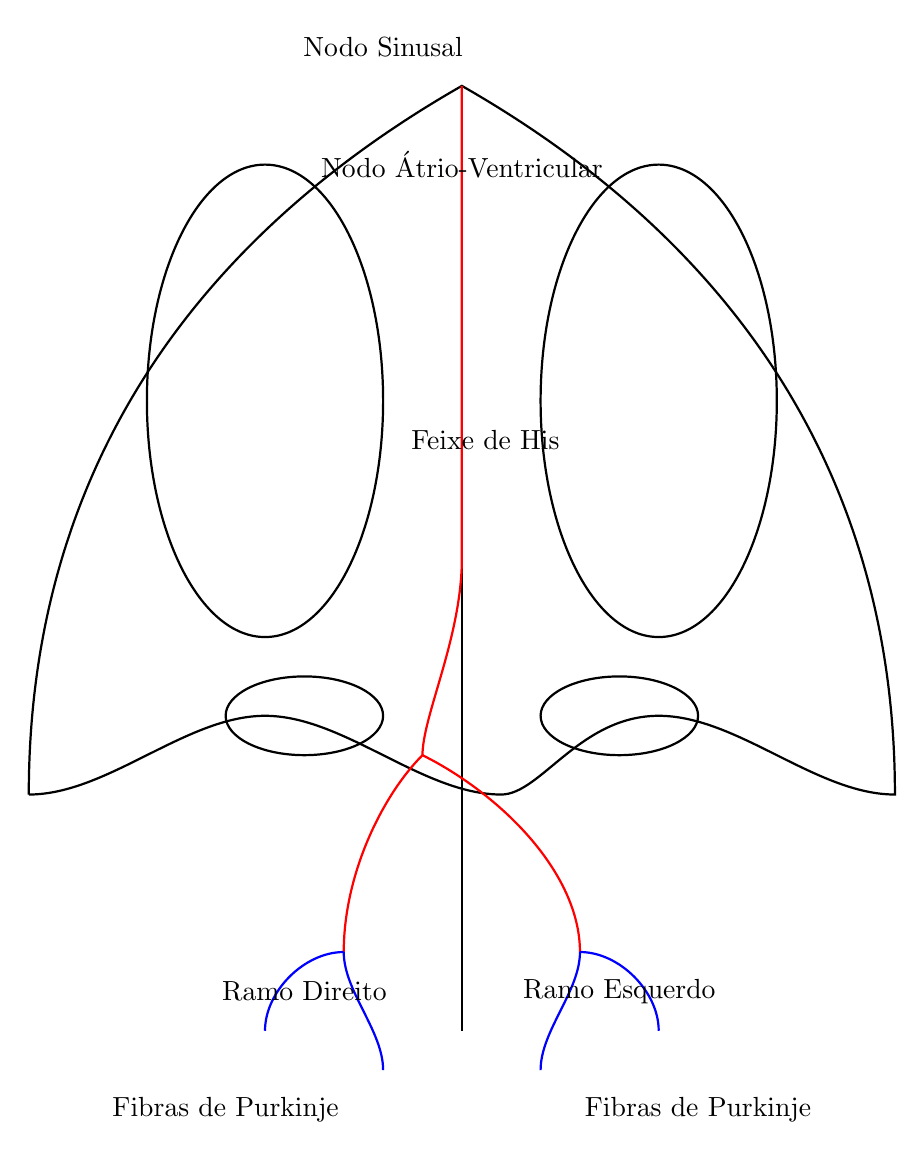
\begin{tikzpicture}
    % Draw miocardio (simplificado)
    \draw[fill=none, thick] (0,3) % miocardio
        .. controls (1,3) and (2,4) .. (3,4)
        .. controls (4,4) and (5,3) .. (6,3)
        .. controls (6.5,3) and (7,4) .. (8,4)
        .. controls (9,4) and (10,3) .. (11,3)
        .. controls (11,7) and (9,10) .. (5.5,12)
        .. controls (2,10) and (0,7) .. (0,3);

    % Draw septum
    \draw[thick] (5.5,12) -- (5.5,0);

    % Draw atria
    \draw[thick, fill=none] (3.5,4) ellipse (1 and 0.5);
    \draw[thick, fill=none] (7.5,4) ellipse (1 and 0.5);

    % Draw ventricles
    \draw[thick, fill=none] (3,8) ellipse (1.5 and 3);
    \draw[thick, fill=none] (8,8) ellipse (1.5 and 3);

    % Draw Feixe de His
    \draw[thick, red] (5.5,12)
        .. controls (5.5,10) and (5.5,8) .. (5.5,6)
        .. controls (5.5,5) and (5,4) .. (5,3.5);

    % Draw Ramo direito
    \draw[thick, red] (5,3.5)
        .. controls (4.5,3) and (4,2) .. (4,1);

    % Draw Ramo esquerdo
    \draw[thick, red] (5,3.5)
        .. controls (6,3) and (7,2) .. (7,1);

    % Draw Fibras de Purkinje (right)
    \draw[thick, blue] (4,1)
        .. controls (3.5,1) and (3,0.5) .. (3,0);
    \draw[thick, blue] (4,1)
        .. controls (4,0.5) and (4.5,0) .. (4.5,-0.5);

    % Draw Fibras de Purkinje (left)
    \draw[thick, blue] (7,1)
        .. controls (7.5,1) and (8,0.5) .. (8,0);
    \draw[thick, blue] (7,1)
        .. controls (7,0.5) and (6.5,0) .. (6.5,-0.5);

    % Labels
    \node at (4.5,12.5) {Nodo Sinusal};
    \node at (5.5,11) {Nodo Átrio-Ventricular};
    \node at (5.8,7.5) {Feixe de His};
    \node at (3.5,0.5) {Ramo Direito};
    \node at (7.5,0.5) {Ramo Esquerdo};
    \node at (2.5,-1) {Fibras de Purkinje};
    \node at (8.5,-1) {Fibras de Purkinje};

\end{tikzpicture}
\end{document}
